In order to use the PSD, two quadrature reference signals are needed. A quadrature generator is an electronical circuit that creates a 90° phase shifted replica of an input signa \cite{Jorgesen2015}. Such a quadrature generator can be created using a comparator and two D-Flip-Flops \cite{horowitz1989art}, as shown in \autoref{fig:QuadratureGenerator}. The comparator creates a square signal that oscillates between $V_{DD}$ and $V_{SS}$, and an inverted version of that signal. Those two signals are sent to the “clock” input of two D-Flip-Flop. The input of the D-Flip-Flops are connected to their own inverted output (effectively transforming the D-Flip-Flop into T-Flip-Flop) \cite{horowitz1989art}. The non-inverted outputs on both Flip-Flop are thus precisely 90° phase shifted from one another, but their frequency is also divided by two compared to the frequency of the signal at the input of the comparator \cite{Jorgesen2015}. \par
\begin{figure}[h]
    \centering
    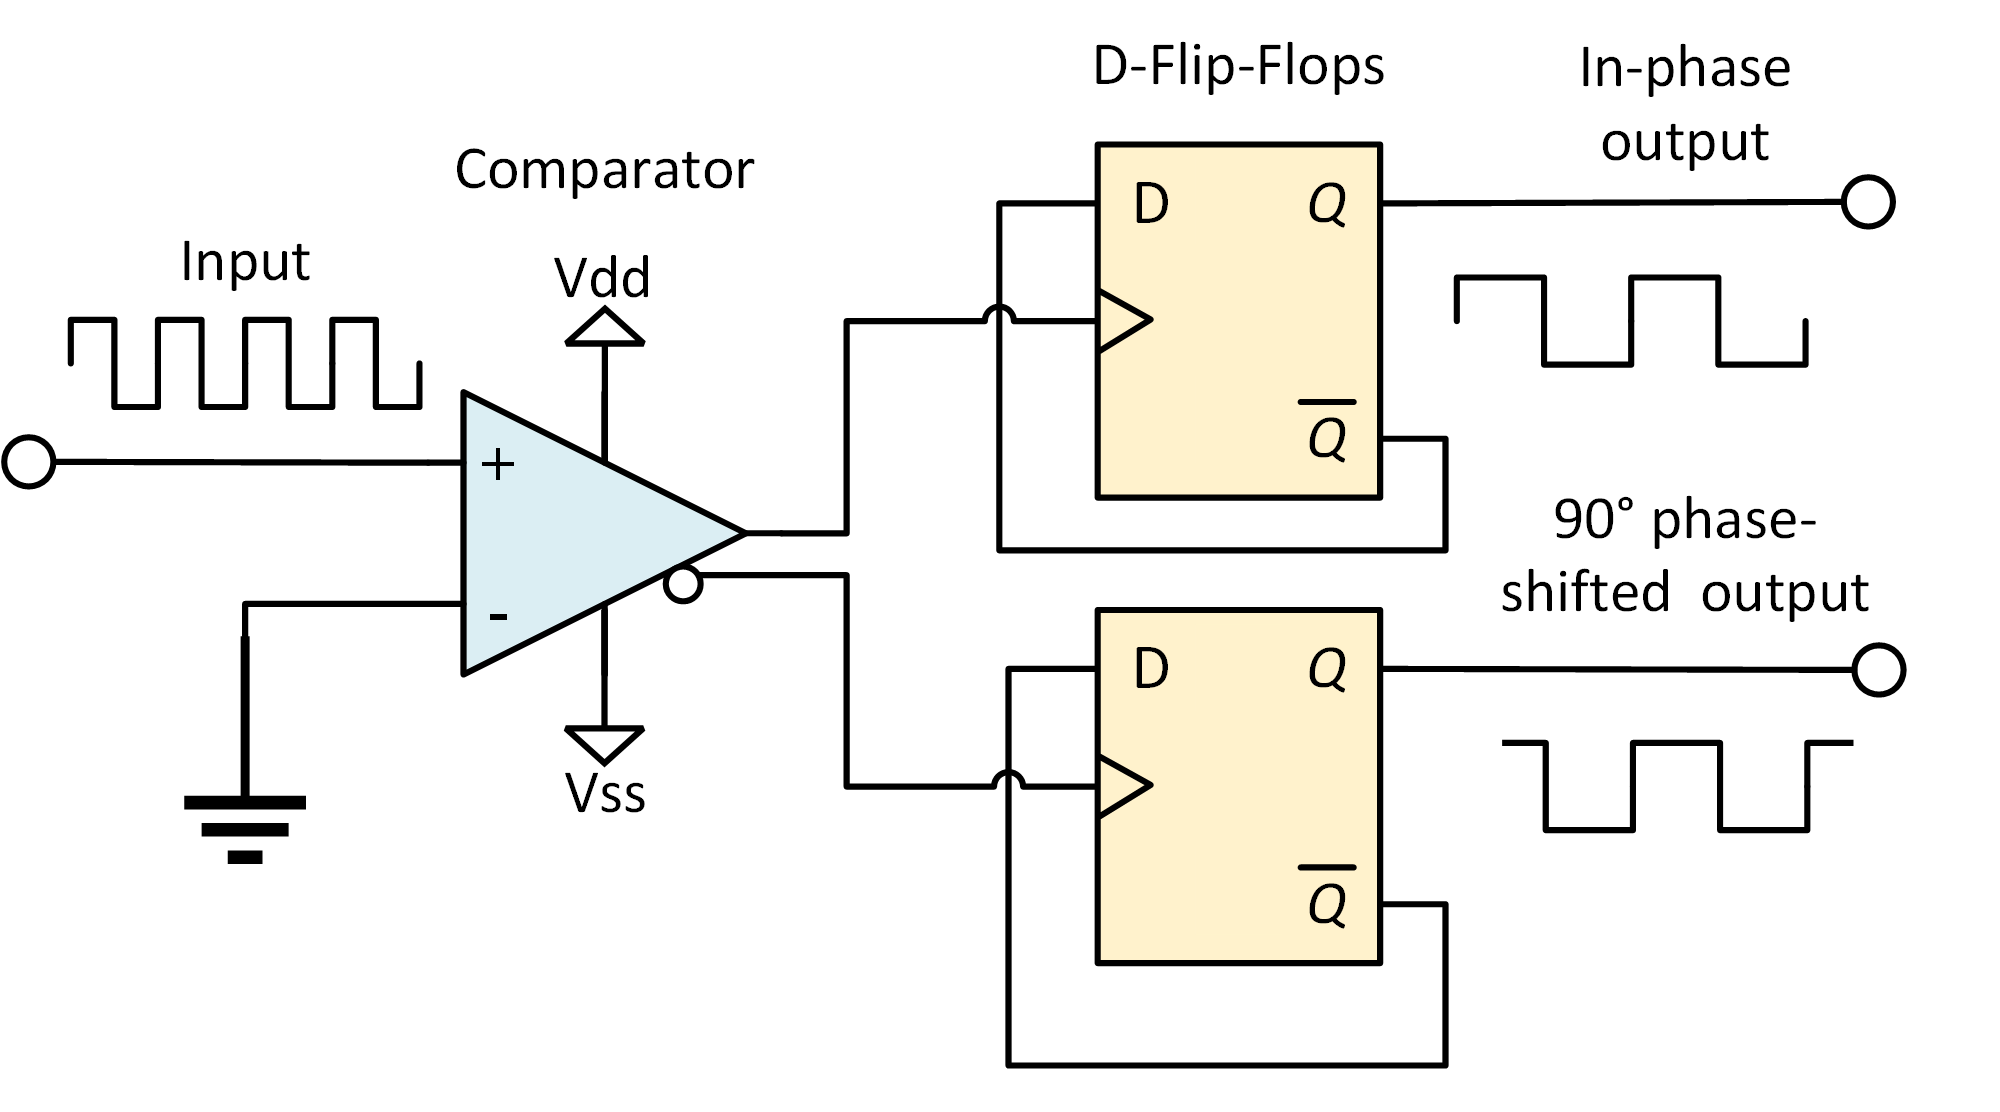
\includegraphics[width=1\textwidth]{QuadratureGenerator}
    \caption{Behavior and implementation of a quadrature generator circuit. Note that the outputs are at half the input frequency.}
    \label{fig:QuadratureGenerator}
\end{figure}
This technique is ultrawideband and relatively simple but can be used only for low-power binary signals. A signal double the output frequency must be provided at the input. They are much affected by duty-cycle errors or phase noise at the input, which are directly seen at the output \cite{Jorgesen2015}.  
